%\documentclass[a4paper,12pt]{article}

%\usepackage{graphics}
%\usepackage[pdftex]{graphicx}

%\begin{document}

\subsection{Topologie de l'Internet}
\par
Commme expliqu\'e pr\'ec\'edemment Internet n'est pas un seul est grand r\'eseau, il s'agit en fait de l'interconnection de plusieurs r\'eseaux ou syst\`emes autonomes (AS). Un syst\`eme autonome est un r\'eseau r\'egit par une administration et soumis \`a un ensemble de r\`egles de routage internes. Les AS sont reli\'es entre eux par diff\'erents types de liens. Ces liens peuvent \^etre de type:
\begin{description}
 \item[PEER] il s'agit d'un accord commercial \`a travers lequel les clients respectifs de deux AS peuvent communiquer entre eux sans que les AS ne doivent se payer la connection,
 \item[P2C ou C2P] il s'agit d'un lien commercial \`a travers lequel un AS devient le client d'un autre et peut faire transf\'erer son trafique r\'eseau.
\end{description}
\par
Au coeur de l'Internet, on trouve les op\'erateurs appel\'es \textit{Tier One} qui sont reli\'es deux \`a deux par des liens de type PEER. Il s'agit l\`a d'une structure type full-mesh aussi appel\'ee \textit{clique} en th\'eorie des graphes. Les \textit{Tier One} sont les grands op\'erateurs qui forment le coeur de l'Internet. Ils en sont en quelque sorte le ciment et les gardiens Ils sont tous reli\'es deux \`a deux par des accords de type PEER, et ne peuvent pas se d\'econnecter. Les \textit{Tier One} peuvent atteindre n'importe quelle destination sur Internet sans avoir \`a payer une seule connection, puisque'\`a plus ou moins au niveau, tout AS est client potentiel d'un \textit{Tier One}. On retrouve parmis les \textit{Tier One} quelques grands nom de télécoms (qui ne sont pas forcément des fournisseurs d'acc\`es) : Orange, Verizon Business, Sprint, AT\&T.
\par
On trouve reli\'es \`a ces grands op\'erateurs d'autres AS qui peuvent eux-m\^eme \^etre reli\'es \`a d'autre et ainsi de suite. De fa\c con locale, on peut retrouver des full-mesh.
\par
Globalement, Internet a une structure connexe, c'est-\`a-dire que si l'on prend deux AS au hasard, il existe un chemin qui les relie.
\par
Il revient \`a chaque AS d'assurer la visibilit\'e de ses clients \`a travers le r\'eseau.
\par
En bout de cha\^ine, il y a des feuilles. Ce sont des AS qui sont clients d'un ou plusieurs autres AS mais qui n'ont pas de client \`a eux. Quand un AS feuille est reli\'e \`a un seul AS, on dit qu'il est \textit{monohom\'e}, si au contraire, il est le client de plusieurs autres AS en m\^eme temps, on dit alors qu'il est \textit{multi-hom\'e}.


\subsubsection{Repr\'esentation d'Internet}
\par
De fa\c con pratique, on peut repr\'esenter Internet comme un graphe o\`u les sommets sont les AS et les ar\^etes les liens entre les AS. La figure suivante montre un exemple de cette repr\'esentation avec un coeur de l'Internet compos\'e de trois AS auxquels sont connect\'es d'autres AS. On remarque que certain AS peuvent \^etre client aupr\`es de plusieurs AS en m\^eme temps. Cette m\'ethode est utile pour garantir un connectivit\'e m\^eme en cas de d\'efaillance d'une connection.

\begin{figure}[ht]
\centering
 \fbox
 {
 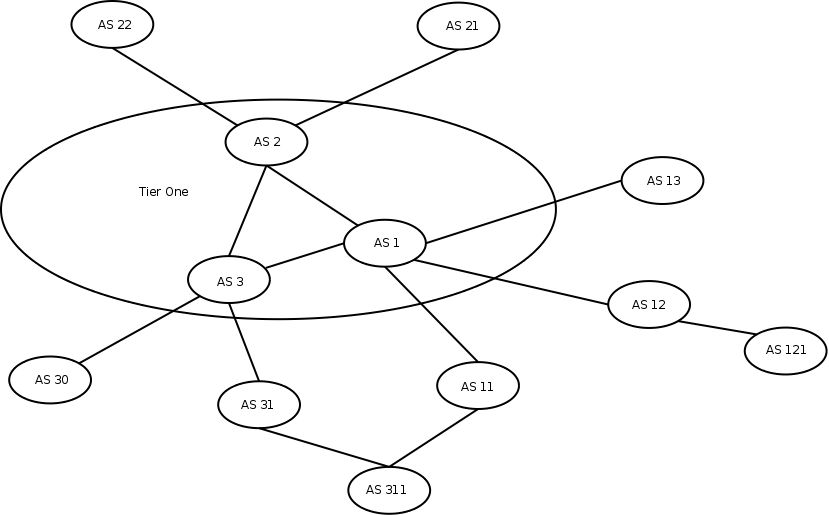
\includegraphics[width=16cm]{./schema/topologie_internet.png}
 }
  \caption{\label{topologie}Topologie d'Internet, exemple de repr\'esentation}
\end{figure}



%\end{document}
